\section{Encodings}
\label{sec:transformation_framework:encodings}
As explained earlier, GROOVE graphs cannot express all elements of Ecore directly. A way to deal with the limitations of GROOVE graphs is by using encodings for these Ecore elements. By encoding, we mean expressing these Ecore model elements as one or more GROOVE graph elements, which preserve all information. The set of GROOVE graph elements then represents a code for the corresponding Ecore element.

\begin{figure}
    \centering
    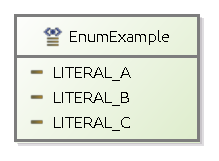
\includegraphics{images/04_transformation_framework/eenum.pdf}
    \caption{Example of an enumeration type in Ecore notation}
    \label{fig:transformation_framework:enumeration_example}
\end{figure}

For example, consider an enumeration type in Ecore, \texttt{EnumExample}, given in \cref{fig:transformation_framework:enumeration_example}. GROOVE has no direct way to express enumerations. However, we can use different encodings to express the enumeration type indirectly. One of such encodings would be to create an abstract node type for the enumeration type and then create a separate node type for each of the values corresponding to the enumeration type. Each of these node types then inherits from the abstract enumeration node type created earlier. An example of this specific encoding is given in \cref{fig:transformation_framework:enumeration_example_groove_encoding_types}. Within an instance graph, each value of an enumeration type is expressed by creating a single node. Each of these nodes is typed by the value node types created earlier. When referencing a value, an edge to the corresponding node can be created.

\begin{figure}
    \centering
    \begin{subfigure}{\textwidth}
        \centering
        % To use this figure in your LaTeX document
% import the package groove/resources/groove2tikz.sty
%
\begin{tikzpicture}[scale=\tikzscale,name prefix=type-]
\node[type_node] (n0) at (4.420, -0.995) {\ml{\textit{\textbf{EnumExample}}}};
\node[type_node] (n1) at (2.040, -0.165) {\ml{\textbf{EnumExample\$LITERAL\_A}}};
\node[type_node] (n2) at (4.420, -0.165) {\ml{\textbf{EnumExample\$LITERAL\_B}}};
\node[type_node] (n3) at (6.800, -0.165) {\ml{\textbf{EnumExample\$LITERAL\_C}}};

\path[subtype_edge] (n1)  --  (n0) ;
\path[subtype_edge](n2.south -| 4.420, -0.995) --  (n0) ;
\path[subtype_edge] (n3)  --  (n0) ;
\end{tikzpicture}

        \caption{GROOVE type graph}
        \label{fig:transformation_framework:enumeration_example_groove_encoding_types:type}
    \end{subfigure}
    \par\medskip
    \begin{subfigure}{\textwidth}
        \centering
        % To use this figure in your LaTeX document
% import the package groove/resources/groove2tikz.sty
%
\begin{tikzpicture}[scale=\tikzscale,name prefix=start-]
\node[basic_node] (n0) at (4.120, -0.170) {\ml{\textbf{EnumExample\$LITERAL\_B}}};
\node[basic_node] (n1) at (6.900, -0.170) {\ml{\textbf{EnumExample\$LITERAL\_C}}};
\node[basic_node] (n2) at (1.340, -0.170) {\ml{\textbf{EnumExample\$LITERAL\_A}}};

\end{tikzpicture}

        \caption{GROOVE instance graph}
        \label{fig:transformation_framework:enumeration_example_groove_encoding_types:instance}
    \end{subfigure}
    \caption{Encoding of the \texttt{EnumExample} enumeration type as different nodes types}
    \label{fig:transformation_framework:enumeration_example_groove_encoding_types}
\end{figure}

Another possible encoding uses flags in GROOVE. In that case, a single node type is created for the enumeration type. This node type gets multiple flags, one for each possible enumeration value. An example of this is shown in \cref{fig:ecore_encodings:enumeration_example_groove_encoding_flags:type}. Within an instance graph, a node is created for each value of the enumeration type. Each of these nodes is typed by the enumeration node type and has a single flag corresponding to the value. An example of these instances is given in \cref{fig:ecore_encodings:enumeration_example_groove_encoding_flags:instance}. This way, each node expresses one value of the enumeration type. When referencing an enumeration value, an edge to the corresponding node can be created.

\begin{figure}
    \centering
    \begin{subfigure}{\textwidth}
        \centering
        % To use this figure in your LaTeX document
% import the package groove/resources/groove2tikz.sty
%
\begin{tikzpicture}[scale=\tikzscale,name prefix=type-]
\node[type_node] (n0) at (0.620, -0.420) {\ml{\textbf{EnumExample}\\\textit{LITERAL\_A}\\\textit{LITERAL\_B}\\\textit{LITERAL\_C}}};

\end{tikzpicture}

        \caption{GROOVE type graph}
        \label{fig:ecore_encodings:enumeration_example_groove_encoding_flags:type}
    \end{subfigure}
    \par\medskip
    \begin{subfigure}{\textwidth}
        \centering
        % To use this figure in your LaTeX document
% import the package groove/resources/groove2tikz.sty
%
\begin{tikzpicture}[scale=\tikzscale,name prefix=start-]
\node[basic_node] (n0) at (1.020, -0.250) {\ml{\textbf{EnumExample}\\\textit{LITERAL\_A}}};
\node[basic_node] (n1) at (2.860, -0.250) {\ml{\textbf{EnumExample}\\\textit{LITERAL\_B}}};
\node[basic_node] (n2) at (4.700, -0.250) {\ml{\textbf{EnumExample}\\\textit{LITERAL\_C}}};

\end{tikzpicture}

        \caption{GROOVE instance graph}
        \label{fig:ecore_encodings:enumeration_example_groove_encoding_flags:instance}
    \end{subfigure}
    \caption{Encoding of the \texttt{EnumExample} enumeration type as one type with multiple flags}
    \label{fig:ecore_encodings:enumeration_example_groove_encoding_flags}
\end{figure}

As the previous examples have shown, creating encodings allows for expressing elements that are unique to Ecore in GROOVE. Moreover, each of these elements might correspond to multiple encodings. The examples for enumeration types presented earlier are non-exhaustive. There are more encodings for enumeration types possible. In other words, there is no single encoding for each element. The choice between different encodings depends on the user, as each encoding might have its advantages and disadvantages.